\documentclass[12pt]{report}

\usepackage{amsmath}
\usepackage{algorithm}
\usepackage{algpseudocode}
\usepackage{float}
\usepackage[standard, thref, hyperref]{ntheorem}
\usepackage{graphicx}
\usepackage{hyperref}
\usepackage{caption}
\usepackage{subcaption}
\usepackage{xeCJK}

\setCJKmainfont{WenQuanYi Zen Hei}

\setlength{\textwidth}{6.5in}
\setlength{\textheight}{8.5in}
\setlength{\evensidemargin}{0in}
\setlength{\oddsidemargin}{0in}
\setlength{\topmargin}{0in}

\setlength{\parindent}{0pt}
\setlength{\parskip}{0.1in}

\begin{document}

\thispagestyle{empty}
\pagenumbering{roman}
\begin{center}

{\Large An Efficient Algorithm for State Propagation on Graph with Lockable Vertices}

\vfill

Yuxiang Lin(林宇翔)

\vfill

Paper for the project submitted to \\
2021 Virginia Tech D.C. Global STEM Expo

\vfill

Keywords: Computer Science, Algorithm, Graph \\
Copyright 2021, Yuxiang Lin, \\
Licensed under Creative Commons Attribution 4.0 International License

\end{center}

\pagebreak

\thispagestyle{empty}
\begin{center}

{\large An Efficient Algorithm for State Propagation on Graph with Lockable Vertices}

\vfill

Yuxiang Lin(林宇翔)

\vfill

(ABSTRACT)

\vfill

\end{center}

There is an interesting class of problems which requires maintaining a binary state carried by each vertex of a graph,
where there also exists an operation where all $ \mathit{true} $ state vertices propagate simultaneously to their $ \mathit{false} $ state neighbors.
And moreover, it is required to be able to lock a vertex from both inbound and outbound state propagation.

This paper will discuss an $ O\left(\lvert V \rvert + q \sqrt{\lvert E \rvert} \right) $ algorithm for such problem, and explore its application.

\pagebreak

\tableofcontents
\pagebreak

\pagenumbering{arabic}
\pagestyle{myheadings}

\chapter{Introduction and Previous Work}
\markright{Yuxiang Lin \hfill Chapter 1. Introduction and Previous Work \hfill}

This algorithm was inspired by a competitive programming problem
\footnote{The contest that provided this problem was an internal contest between a few schools, and I was unable to recover the name of its author.}
that has a background of modelling the transmission of virus,
which is stated as such, given a \textbf{tree} with each vertex holding two boolean variables,
$ s $ (e.g. \textbf{infected} or \textbf{not infected}) and $ \mathit{locked} $ (e.g. \textbf{under lockdown} or \textbf{not under lockdown}), and the following operations must be implemented:

\begin{description}
	\item [$ \mathrm{set}(\mathbf{vertex}\ v) $] Let $ v.s \gets \mathit{true} $.
	\item [$ \mathrm{flip}(\mathbf{vertex}\ v) $] Flip $ v.\mathit{locked} $.
	\item [$ \mathrm{propagate}() $] \sloppy For each pair of neighboring vertices $ v_0 $ and $ v_1 $, where $ v_0.s = \mathit{true} $ and $ v_0.\mathit{locked} = \mathit{false} $,
		and $ v_1.s = \mathit{false} $ and $ v_1.\mathit{locked} = \mathit{false} $, let $ v_1.s \gets \mathit{true} $.
\end{description}

This problem can be solved in $ \Theta\left(\lvert V \rvert + q \right) $ time, where $ q $ is the total number of calls to all three functions.
Since the process of communicating states is between two vertices, but the propagation operation is applied by one to another,
it would be sensible to have the vertex initiating such operation iterate through as few neighbors as possible.
Then consider the fact that for each vertex on a tree, a fixed parent can be appointed for it.

\bigskip

Let's refer to a vertex $ v $ where $ v.s = \mathit{true} $ and $ v.\mathit{locked} = \mathit{false} $ as a \textbf{source}, and a vertex where $ v.s = \mathit{false} $ and $ v.\mathit{locked} = \mathit{false} $ as a \textbf{target}. \\
So the outline of the algorithm is:
\begin{itemize}
	\item Fix the root of the tree.
	\item Have each vertex becoming a \textbf{source} or a \textbf{target} add itself to a global queue.
	\item Have each vertex becoming or no longer being a \textbf{source} increase or decrease a counter variable owned by its parent respectively.
	\item Have each vertex becoming a \textbf{target} add itself to a queue owned by its parent.
	\item During the propagation process, go through the global queue;
		  for each \textbf{source} vertex, propagate to its parent and each vertex in its queue that is a \textbf{target};
		  and for each \textbf{target} vertex, check whether its parent is a \textbf{source} or its counter variable is a positive number,
		  and update accordingly.
	\item Both the global and vertex-owned queue will be cleared afterwards.
\end{itemize}


Note that although the vertex that became a \textbf{source} or \textbf{target} can revert its state after its inclusion into the queues, the number of pop operation is bounded by the number of push operations in a queue.

Now it is important to know that the major difference between the problem stated above and the problem I aim to solve is that whereas a \textbf{tree} was given above, my algorithm will be applicable to any \textbf{graph}.

\pagebreak

\chapter{The Algorithm}
\markright{Yuxiang Lin \hfill Chapter 2. The Algorithm \hfill}

\section{The Algorithm}
Now let's extend the algorithm to any \textbf{undirected graph},
with $ \mathrm{set}(\mathbf{vertex}\ v, \mathbf{bool}\ s') $ and $ \mathrm{setLock}(\mathbf{vertex}\ v, \mathbf{bool}\ \mathit{locked}') $ to be implemented.
The parameters are a little different from the ones in the introduction,
since the caller actually knows the assumed state of the program for a competitive programming algorithm, whereas this algorithm does not assume such.

To design an algorithm for any undirected graph, its most prominent issue would be the varying degrees of the vertices,
since the naive algorithm will suffer a huge time penalty during a state update to a vertex with a large degree (\textbf{large} vertex for short).
Recall the idea of having each vertex communicate with its parent when the graph is a tree,
so it would be intuitive to appoint some kind of ``parent equivalent" for a vertex on any graph.
Also to note is that the number of large vertices is rather small due to its number being bounded by the degree of the graph.
So let's define a critical constant for the graph $ \mathit{crit} $, then for any vertex $ v $ with $ v.\mathit{degree} > \mathit{crit} $,
it would be considered a \textbf{large} vertex,
in another word, a ``parent equivalent" for all its neighbors (including other large neighbors).
Thus for all $ \mathrm{set}() $ and $ \mathrm{setLock}() $ operations, the vertex acted upon shall notify all its large neighbors (even if the vertex itself is a large vertex).
\ref{tbl:vert_int} gives a summary of how different vertices interact with their neighbors when being acted on.

\begin{table}[h]
\footnotesize
\centering
\begin{tabular}{|l|l|l|}
	\hline
				 & $ \mathrm{set}() $ and $ \mathrm{setLock}() $ & $ \mathrm{propagate}() $                                \\ \hline
	small vertex & notify all large neighbors                    & iterate through all neighbors                           \\ \hline
	large vertex & notify all large neighbors                    & iterate through queues of potential sources and targets \\ \hline
\end{tabular}
\caption{Vertex interaction with neighbors when being acted on.}
\label{tbl:vert_int}
\end{table}

With these ideas, the algorithm is given below with the minimum total time complexity of $ O\left(\lvert V \rvert + q \sqrt{\lvert E \rvert} \right) $ for $ \mathit{crit} = \Theta(\sqrt{\lvert E \rvert}) $.
This technique of separating small items of large quantity and large items of small quantity is similar to the meet-in-the-middle technique popularized by its application in the Baby-step Giant-step algorithm.\cite{shanks71}

\bigskip

At the beginning of the program, $ \mathrm{initialize}() $ is called once with $ v.\mathit{adj} $ being an array of vertices reached by edges of $ v $, then any of the three functions can be called each time for a total of $ q $ times

\begin{algorithm}[H]
\caption{Initialize}
\begin{algorithmic}
\For{each $ v $}
	\State $ v.s \gets \mathit{false} $
	\State $ v.\mathit{locked} \gets \mathit{false} $
	\\
	\For{each $ v' $ in $ v.\mathit{adj} $}
		\If{$ v'.\mathit{degree} > \mathit{crit} $}
			\State $ v.\mathit{large}.\mathrm{pushBack}(v') $
			\State $ v'.\mathit{targets}.\mathrm{pushBack}(v) $
		\EndIf
	\EndFor
\EndFor
\end{algorithmic}
\end{algorithm}

\begin{algorithm}[H]
\caption{Set}
\begin{algorithmic}
\Require $ \mathbf{vertex}\ v, \mathbf{bool}\ s' $
\If{$ v.s = s' \lor v.\mathit{locked} $}
	\State \Return
\EndIf
\State $ v.s \gets s' $
\\
\If{$ v.s $}
	\For{each $ v' $ in $ v.\mathit{large} $}
		\State $ v'.\mathit{sources} \gets v'.\mathit{sources} + 1 $
	\EndFor
\Else
	\For{each $ v' $ in $ v.\mathit{large} $}
		\State $ v'.\mathit{sources} \gets v'.\mathit{sources} - 1 $
		\State $ v'.\mathit{targets}.\mathrm{pushBack}(v) $
	\EndFor
\EndIf
\State $ \mathit{queue}.\mathrm{pushBack}(v) $
\end{algorithmic}
\end{algorithm}

\begin{Lemma}
The time complexity of $ \mathrm{set}() $ is $ O(\frac{\lvert E \rvert}{\mathit{crit}}) $.
\label{thm:set}
\end{Lemma}
\begin{Proof}
	For each vertex $ v' $ in $ v.\mathit{large} $, it must satisfy that $ v'.\mathit{degree} > \mathit{crit} $. \\
	Since the total degree of an undirected graph is $ 2 \lvert E \rvert $, the number of large vertices is at most $ \frac{2 \lvert E \rvert}{\mathit{crit}} $.
\end{Proof}

\begin{algorithm}[H]
\caption {setLock}
\begin{algorithmic}
\Require $ \mathbf{vertex}\ v, \mathbf{bool}\ \mathit{locked}'$
\If{$ v.\mathit{locked} = \mathit{locked}' $}
	\State \Return
\EndIf
\State $ v.\mathit{locked} \gets v.\mathit{locked}' $
\\
\If{$ v.\mathit{locked} $}
	\If{$ v.s $}
		\For{each $ v' $ in $ v.\mathit{large} $}
			\State $ v'.\mathit{sources} \gets v'.\mathit{sources} - 1 $
		\EndFor
	\EndIf
\Else
	\If{$ v.s $}
		\For{each $ v' $ in $ v.\mathit{large} $}
			\State $ v'.\mathit{sources} \gets v'.\mathit{sources} + 1 $
		\EndFor
	\Else
		\For{each $ v' $ in $ v.\mathit{large} $}
			\State $ v'.\mathit{targets}.\mathrm{pushBack}(v) $
		\EndFor
	\EndIf
	\State $ \mathit{queue}.\mathrm{pushBack}(v) $
\EndIf
\end{algorithmic}
\end{algorithm}

\begin{Lemma}
The time complexity of $ \mathrm{setLock}() $ is $ O(\frac{\lvert E \rvert}{\mathit{crit}}) $.
\end{Lemma}
\begin{Proof}
This is proved the same as \thref{thm:set}.
\end{Proof}

\begin{algorithm}[H]
\caption{Propagate}
\begin{algorithmic}
\State Declare empty temporary queues $ \mathit{temp} $ and $ \mathit{pending} $
\State $ \mathrm{swap}(\mathit{queue}, \mathit{temp}) $
\For{each $ v $ in $ \mathit{temp} $}
	\If{$ v.\mathit{locked} $}
		\State \textbf{continue}
	\EndIf
	\\
	\If{$ v.s $}
		\If{$ v.\mathit{degree} > \mathit{crit} $}
			\For{each $ v' $ in $ v.\mathit{targets} $}
				\State $ \mathit{pending}.\mathrm{pushBack}(v') $
			\EndFor
			\State $ v.\mathit{targets}.\mathrm{clear}() $
		\Else
			\For{each $ v' $ in $ v.\mathit{adj} $}
				\State $ \mathit{pending}.\mathrm{pushBack}(v') $
			\EndFor
		\EndIf
	\Else
		\If{$ v.\mathit{degree} > \mathit{crit} $}
			\If{$ v.\mathit{sources} > 0 $}
				\State $ \mathit{pending}.\mathrm{pushBack}(v) $
			\EndIf
		\Else
			\For{each $ v' $ in $ v.\mathit{adj} $}
				\If{$ \neg v'.\mathit{locked} \land v'.s $}
					\State $ \mathit{pending}.\mathrm{pushBack}(v) $
					\State \textbf{break}
				\EndIf
			\EndFor
		\EndIf
	\EndIf
\EndFor
\\
\For {each $ v $ in $ \mathit{pending} $}
	\State $ \mathrm{set}(v, \textit{true}) $
\EndFor
\end{algorithmic}
\end{algorithm}

\begin{Lemma}
The total amortized time complexity of $ \mathrm{propagate}() $ is $ O\left(\lvert V \rvert + q \cdot \left(\mathit{crit} + \frac{\lvert E \rvert}{\mathit{crit}} \right) \right) $.
\end{Lemma}
\begin{Proof}
First of all, $ \lvert V \rvert $ targets are pushed into vertex-owned queue by $ \mathrm{init}() $. \\
For each call to $ \mathrm{set}() $ and $ \mathrm{setLock}() $, at most one vertex is pushed into the global queue. \\
For each call to $ \mathrm{setLock}() $, the current vertex might be pushed into $ O(\frac{\lvert E \rvert}{\mathit{crit}}) $ vertex-owned queues. \\
For each vertex $ v $ with $ v.\mathit{locked} = \mathit{false} $ in the global queue,
if it is a large vertex with $ v.s = \mathit{true} $, then the run time of $ \mathrm{propagate}() $ will bounded by the size of $ v.\mathit{targets} $;
and if it is a small vertex, it will go through all its neighbors, which there are, $ O(\mathit{crit}) $ of them.
\end{Proof}

\begin{Corollary}
The total time complexity of the algorithm is $ O\left(\lvert V \rvert + q \cdot \left(\mathit{crit} + \frac{\lvert E \rvert}{\mathit{crit}} \right) \right) $.
\end{Corollary}

\begin{Theorem}
The minimum total time complexity of the algorithm is $ O\left(\lvert V \rvert + q \sqrt{\lvert E \rvert} \right) $ for $ \mathit{crit} = \Theta(\sqrt{\lvert E \rvert}) $.
\end{Theorem}
\begin{Proof}
Easily proved by basic inequality $ \mathit{crit} + \frac{\lvert E \rvert}{\mathit{crit}} \ge 2 \sqrt{\lvert E \rvert} $,
with $ \mathit{crit} + \frac{\lvert E \rvert}{\mathit{crit}} = 2 \sqrt{\lvert E \rvert} $ only when $ \mathit{crit} = \sqrt{\lvert E \rvert}. $
\end{Proof}

\pagebreak

\section{Example}

\begin{figure}[H]
\centering
\begin{subfigure}{0.45\textwidth}
	\includegraphics[width=0.7\textwidth,angle=-90]{graph/example/0.eps}
	\caption{$ \mathrm{set}(0, \mathit{true}) $}
\end{subfigure}
\begin{subfigure}{0.45\textwidth}
	\includegraphics[width=0.7\textwidth,angle=-90]{graph/example/1.eps}
	\caption{$ \mathrm{setLock}(5, \mathit{true}) $}
\end{subfigure}
\\
\begin{subfigure}{0.45\textwidth}
	\includegraphics[width=0.7\textwidth,angle=-90]{graph/example/2.eps}
	\caption{$ \mathrm{propagate}() $}
\end{subfigure}
\begin{subfigure}{0.45\textwidth}
	\includegraphics[width=0.7\textwidth,angle=-90]{graph/example/3.eps}
	\caption{$ \mathrm{setLock}(5, \mathit{false}) $}
\end{subfigure}
\\
\begin{subfigure}{0.45\textwidth}
	\includegraphics[width=0.7\textwidth,angle=-90]{graph/example/4.eps}
	\caption{$ \mathrm{setLock}(3, \mathit{true}) $}
\end{subfigure}
\begin{subfigure}{0.45\textwidth}
	\includegraphics[width=0.7\textwidth,angle=-90]{graph/example/5.eps}
	\caption{$ \mathrm{propagate}() $}
\end{subfigure}

\caption{An example for $ \lvert V \rvert = 8, \lvert E \rvert = 15, q = 6 $,
         with the size of the vertex mark denoting whether it is a large vertex,
         and the color of light blue and orange for $ v.s = 0 $ and $ v.s = 1 $ respectively.}
\end{figure}

\chapter{Experiments}
\markright{Yuxiang Lin \hfill Chapter 3. Experiments \hfill}

The following experiments are all done with C++ implementations compiled with Clang 11.0.1 (no optimization flags),
and run on a PC with Intel(R) Core(TM) i7-8750H CPU @ 2.20 GHz (max turbo frequency 4.10 GHz) and 32026.3 MiB RAM,
the operating system is Debian GNU/Linux bullseye/sid.

Two kinds of graphs are used for the experiment:
\begin{itemize}
	\item The $ G(n, m) $ \textbf{model} of the \textbf{Erdős–Rényi model},
		  which is a random graph out of all possible graphs with $ n $ vertices and $ m $ edges,
		  it will be referred to as $ G_\mathrm{rand}(n, m) $ below.\cite{er59}
	\item The \textbf{Barabási–Albert model},
		  which generates a graph of $ n $ vertices by adding vertices incrementally,
		  with each new vertex creating edges to $ m $ known vertices,
		  and the old vertices' probability to connect to the new vertex is proportional to its degree,
		  it will be referred to as $ G_\mathrm{BA}(n, m) $ below.\cite{ba02}
\end{itemize}

The graphs generated are assumed to have no self-loops and duplicated edges.
In implementation, a $ G_\mathrm{rand} $ is generated by adding $ m $ edges with two random end vertices.
And a $ G_\mathrm{BA} $ is generated by initially choose $ m $ known vertices,
and for each of the rest of the vertices it will create $ m $ random edges to known vertices,
where the probabilty to connect to a known vertex $ v $ out of any known vertex $ i $ is: $ p_v = \frac{w_v}{\sum_i w_i} $,
then it will be added the known vertices;
$ w_v $ is set to $ 1 $ for each initial vertex $ v $, otherwise $ w_v \gets 0 $,
then $ w_v $ is incremented for the endpoints of each edge added.

The $ q $ operations generated are of random type,
and for $ \mathrm{set}() $ and $ \mathrm{setLock}() $, $ s' $ and $ \mathit{locked}' $ are also random.
What to note is that $ v $ will be random, but is of some discrete distribution specified below.

\sloppy The two kinds of graphs I will use below will now be specifically $ G_\mathrm{rand}(10^6, 10^7) $ and $ G_\mathrm{BA}(10^6, 10) $,
they were chosen for their moderately large size and sparseness,
and they also have approximately same number of edges.

It was found that for a graph of either type, when all vertices are initially unlocked,
it will just take very few ($ < 50 $) instructions for almost all vertices have $ v.s = \mathit{true} $.
So before the random operations, $ n $ $ \mathrm{setLock}() $ operations will be generated,
iterating through all vertices, and $ 0.1 $ of the operations will have $ \mathit{locked}' = \mathit{true} $.
These operations will not be counted in the $ q $ operations,
so $ n + q $ operations will be executed \textit{de facto}.
Note that this still meant a large amount of vertices will have $ v.s = \mathit{true} $ after the first few instructions,
but then the speed of propagation will slow down.

\begin{figure}
\centering
\begin{subfigure}{0.45\textwidth}
	\includegraphics[width=0.7\textwidth,angle=-90]{graph/uniform_coverage_1000000_10000000_0.eps}
	\caption{$ G_\mathrm{rand}(10^6, 10^7) $}
\end{subfigure}
\begin{subfigure}{0.45\textwidth}
	\includegraphics[width=0.7\textwidth,angle=-90]{graph/ba_coverage_1000000_10_0.eps}
	\caption{$ G_\mathrm{BA}(10^6, 10) $}
\end{subfigure}
\caption{Number of $ v.s = \mathit{true} $ after executing $ q $ operations when all vertices are initially unlocked,
	     tests done by repeating on $ 5 $ graphs and $ 5 $ sets of operations for each graph and averaging the results..}
\end{figure}

I first pit the algorithm mentioned in this paper (the ``novel" algorithm) against the ``naive" implementation.
The naive algorithm is implemented by having each $ \mathrm{set}() $ and $ \mathrm{setLock}() $ function add the current vertex to the global queue,
and $ \mathrm{propagate}() $ function will go through all neighbors of the current vertex.

It was found that in order for the novel algorithm to perform better than the naive implementation,
it will be necessary to access vertices of higher degree much more often.
So the $ v $ generated in an operation will be of a discrete distribution
that the probability where vertex $ v $ is chosen out of any vertex $ i $ is: $ p_v = \frac{w_v}{\sum_i w_i} $.
I attempted to set the weight to be equal to the degree of the vertex,
it was also attempted to have it to equal to some measures of graph centralities: betweenness, PageRank, and lobby index,
which may be of some legitimate applicational implications,
but the results are all unsatisfying.\cite{freeman77}\cite{bp98}\cite{kst09}

But I found that for $ G_\mathrm{BA}(10^6, 10) $, when setting $ w_v = \mathit{deg}_v^a $, for some small $ a \ge 3 $,
the novel algorithm will run faster.
It was also tried to set $ w_v = a^{\mathit{deg}_v} $,
but then a unreasonably large weight would be given to too few vertices,
and the entire process will just focus on them.
It was as expected that the algorithm didn't run faster on $ G_\mathrm{rand}(10^6, 10^7) $ even when vertices are weighted,
since its degree distribution is approximately a normal distribution with almost no large vertices;
but for a Barabási–Albert graph, its degree distribution in its tail follows a power law so that $ P(x) \sim x^{-3} $ for some degree $ x $,
so there will be, even though few, large vertices.

\begin{figure}
\centering
\begin{subfigure}{0.45\textwidth}
	\includegraphics[width=0.7\textwidth,angle=-90]{graph/uniform_degree.eps}
	\caption{$ G_\mathrm{rand}(10^6, 10^7) $}
\end{subfigure}
\begin{subfigure}{0.45\textwidth}
	\includegraphics[width=0.7\textwidth,angle=-90]{graph/ba_degree.eps}
	\caption{$ G_\mathrm{BA}(10^6, 10) $}
\end{subfigure}
\caption{The degree distribution of a randomly generated graph from each of two kinds of graphs.}
\end{figure}

The results for both kind of graphs are shown here for no weight, degree as weight, and power of degree as weight, all setting $ \mathit{crit} = \sqrt{m} $.
Note that running time begins from non-zero, since the execution of the initial $ n $ instructions were taken into account.
It can also be observed that when the input is unfavorable to the novel algorithm,
if initialization time is ignored, the time difference will be negligible.

\begin{figure}
\centering
\begin{subfigure}{0.35\textwidth}
	\includegraphics[width=0.7\textwidth,angle=-90]{graph/uniform_coverage_1000000_10000000_0.1.eps}
	\caption{All $ w_v $ are equal}
\end{subfigure}
\begin{subfigure}{0.35\textwidth}
	\includegraphics[width=0.7\textwidth,angle=-90]{graph/uniform_q_1000000_10000000_0.1.eps}
	\caption{All $ w_v $ are equal}
\end{subfigure}

\begin{subfigure}{0.35\textwidth}
	\includegraphics[width=0.7\textwidth,angle=-90]{graph/uniform_coverage_1000000_10000000_0.1_power_1.eps}
	\caption{$ w_v = \mathit{deg}_v $}
\end{subfigure}
\begin{subfigure}{0.35\textwidth}
	\includegraphics[width=0.7\textwidth,angle=-90]{graph/uniform_q_1000000_10000000_0.1_power_1.eps}
	\caption{$ w_v = \mathit{deg}_v $}
\end{subfigure}

\begin{subfigure}{0.35\textwidth}
	\includegraphics[width=0.7\textwidth,angle=-90]{graph/uniform_coverage_1000000_10000000_0.1_power_2.eps}
	\caption{$ w_v = \mathit{deg}_v^2 $}
\end{subfigure}
\begin{subfigure}{0.35\textwidth}
	\includegraphics[width=0.7\textwidth,angle=-90]{graph/uniform_q_1000000_10000000_0.1_power_2.eps}
	\caption{$ w_v = \mathit{deg}_v^2 $}
\end{subfigure}

\begin{subfigure}{0.35\textwidth}
	\includegraphics[width=0.7\textwidth,angle=-90]{graph/uniform_coverage_1000000_10000000_0.1_power_3.eps}
	\caption{$ w_v = \mathit{deg}_v^3 $}
\end{subfigure}
\begin{subfigure}{0.35\textwidth}
	\includegraphics[width=0.7\textwidth,angle=-90]{graph/uniform_q_1000000_10000000_0.1_power_3.eps}
	\caption{$ w_v = \mathit{deg}_v^3 $}
\end{subfigure}
	\caption{Left: number of $ v.s = \textit{true} $ after executing $ q $ operations on $ G_\mathrm{rand}(10^6, 10^7) $;
	         Right: time in seconds after executing $ q $ operations on $ G_\mathrm{rand}(10^6, 10^7) $;
			 All tests done by repeating on $ 5 $ graphs and $ 5 $ sets of operations for each graph and averaging the results.}
\end{figure}

\begin{figure}
\centering
\begin{subfigure}{0.35\textwidth}
	\includegraphics[width=0.7\textwidth,angle=-90]{graph/ba_coverage_1000000_10_0.1.eps}
	\caption{All $ w_v $ are equal}
\end{subfigure}
\begin{subfigure}{0.35\textwidth}
	\includegraphics[width=0.7\textwidth,angle=-90]{graph/ba_q_1000000_10_0.1.eps}
	\caption{All $ w_v $ are equal}
\end{subfigure}

\begin{subfigure}{0.35\textwidth}
	\includegraphics[width=0.7\textwidth,angle=-90]{graph/ba_coverage_1000000_10_0.1_power_1.eps}
	\caption{$ w_v = \mathit{deg}_v $}
\end{subfigure}
\begin{subfigure}{0.35\textwidth}
	\includegraphics[width=0.7\textwidth,angle=-90]{graph/ba_q_1000000_10_0.1_power_1.eps}
	\caption{$ w_v = \mathit{deg}_v $}
\end{subfigure}

\begin{subfigure}{0.35\textwidth}
	\includegraphics[width=0.7\textwidth,angle=-90]{graph/ba_coverage_1000000_10_0.1_power_2.eps}
	\caption{$ w_v = \mathit{deg}_v^2 $}
\end{subfigure}
\begin{subfigure}{0.35\textwidth}
	\includegraphics[width=0.7\textwidth,angle=-90]{graph/ba_q_1000000_10_0.1_power_2.eps}
	\caption{$ w_v = \mathit{deg}_v^2 $}
\end{subfigure}

\begin{subfigure}{0.35\textwidth}
	\includegraphics[width=0.7\textwidth,angle=-90]{graph/ba_coverage_1000000_10_0.1_power_3.eps}
	\caption{$ w_v = \mathit{deg}_v^3 $}
\end{subfigure}
\begin{subfigure}{0.35\textwidth}
	\includegraphics[width=0.7\textwidth,angle=-90]{graph/ba_q_1000000_10_0.1_power_3.eps}
	\caption{$ w_v = \mathit{deg}_v^3 $}
\end{subfigure}
	\caption{Left: number of $ v.s = \textit{true} $ after executing $ q $ operations on $ G_\mathrm{BA}(10^6, 10) $;
	         Right: time in seconds after executing $ q $ operations on $ G_\mathrm{BA}(10^6, 10) $;
			 All tests done by repeating on $ 5 $ graphs and $ 5 $ sets of operations for each graph and averaging the results.}
\end{figure}

It was also attempted to find the optimal $ \mathit{crit} $ value,
but I am unable to find a clear trend of running time for varying $ \mathit{crit} $.

\begin{figure}
\centering
\includegraphics[width=2.2in,angle=-90]{graph/ba_crit_power.eps}
\caption{Time in seconds for varying $ a $ and $ r $; for each data point, let $ w_v = \mathit{deg}_v^a $ and $ \mathit{crit} = r \sqrt{m} $, then execute $ 10^6 $ operations on $ G_\mathrm{BA}(10^6, 10) $; tests done by repeating on $ 7 $ graphs and $ 7 $ sets of operations for each graph and averaging the results.}
\end{figure}

\pagebreak

\chapter{Applications and Modifications}
\markright{Yuxiang Lin \hfill Chapter 4. Applications \hfill}

I suspect this algorithm might have some use in machine learning and artificial neural networks,
but I was yet to find a case that might require locking the states of vertices.
I do observe that the technique of \textbf{label propagation} bears some similarity to this problem.\cite{zhu02}
But instead of going from a $ \mathit{false} $ state to a $ \mathit{true} $ state,
states can now be of many different labels,
but that does not change the nature of the problem since the states always go from null label to some label.
What it was really lacking was the need to lock the states of vertices.

This algorithm could also have some applications on the transmission of information on graphs of interpersonal ties,
for their nature of being approximately Barabási-Albert graphs,
and locking the vertices could represent that some persons are unavailable.\cite{granovetter05}
Also to note is that more ``influential" persons (vertices of large degree) tend to be more active,
so this might give my algorithm an edge over the naive one.

A similar application would be modelling the spreading of disease, which was also the algorithm's original background.\cite{aay21}
In this case, locking a vertex can represent the variables that prevent disease transmission.
But such problem is much more complicated since more variables need to be taken into consideration,
the edges now may have weights, and each vertex could be in one of many different states with some criteria to enter another state.
Such simulation will also take time into consideration.
Thus it would be necessary for the algorithm to have some kind of event processing,
and the queues will store timestamp to allow simulation in time steps.

\pagebreak

\chapter{Conclusions}
\markright{Yuxiang Lin \hfill Chapter 5. Conclusions \hfill}

This paper described an algorithm to simulate state propagation on graph while allowing the vertices to be locked.
It was also found that this algorithm will perform better than the naive implementation only when vertices of high degree were accessed much more often.
Some possible applications were discussed about this algorithm.
How exactly weighing the vertices by the power of their degrees will be applicable,
the better ways to find the optimal $ \mathit{crit} $ value,
and how the probability distribution of the type of the operations will affect the performance of this algorithm will be left for further studies.
It might also be good to have an adaptive version of the algorithm to increase its performance in different situations better.

\pagebreak

\begin{thebibliography}{9}

\bibitem{shanks71}
	D. Shanks,
	Class number, a theory of factorization and genera,
	Proc. Symp. Pure Math,
	20,
	Pages 415—440.
	AMS, Providence, R.I.,
	1971.

\bibitem{er59}
	Erdős, P.; Rényi, A,
	On Random Graphs. I,
	Publicationes Mathematicae,
	6,
	Pages 290–297,
	1959.

\bibitem{ba02}
	Albert, Réka; Barabási, Albert-László,
	Statistical mechanics of complex networks,
	Reviews of Modern Physics,
	74 (1),
	Pages 47–97,
	2002.

\bibitem{freeman77}
	Freeman, Linton,
	A set of measures of centrality based on betweenness,
	Sociometry,
	40 (1),
	Pages 35–41,
	1977.

\bibitem{bp98}
	Brin, S.; Page, L.,
	The anatomy of a large-scale hypertextual Web search engine,
	Computer Networks and ISDN Systems,
	30 (1–7),
	Pages 107–117,
	1998.

\bibitem{kst09}
	Korn, A.; Schubert, A.; Telcs, A.,
	Lobby index in networks,
	Physica A,
	388 (11),
	Pages 2221–2226,
	2009.

\bibitem{zhu02}
	Zhu, Xiaojin,
	Learning From Labeled and Unlabeled Data With Label Propagation,
	2002.

\bibitem{granovetter05}
	Granovetter, Mark,
	The Impact of Social Structure on Economic Outcomes,
	Journal of Economic Perspectives,
	19 (1),
	Pages 33–50,
	2005.

\bibitem{aay21}
	Rasim Alguliyev, Ramiz Aliguliyev, Farhad Yusifov,
	Graph modelling for tracking the COVID-19 pandemic spread,
	Infectious Disease Modelling,
	Volume 6,
	Pages 112-122,
	2021.

\end{thebibliography}

\end{document}
